\documentclass[10pt]{article}
\usepackage{pdfpages}

\title{\textbf{DASH} \\Documentation}
\date{January 22, 2015}
\author{Zachary Pierson}

\begin{document}
\maketitle

\par\vspace{\fill}%push the table of contents to the bottom of the page
\tableofcontents
\newpage

\section{Introduction}
\paragraph{}
dash is a program that enters a Read Eval Print Loop and allows
the user to find information on certain processes.  

\subsection{Usage}
\subparagraph{}
This is a new Subsection of the Introduction

\section{How To}
\paragraph{}
This paragraph will talk about everything you need to know

\section{Another Section}
\paragraph{}
Another section we will talk about will include a lot of interesting and promising things about our talk.

\subsection{Another Subsection}
\subparagraph{}
A SUB PARAGRAPH!

\newpage
\section{APPENDICES}
\appendix

\subsection{Source Code}

\subsection{Program Assignment}
%\label{App:AppendixA}
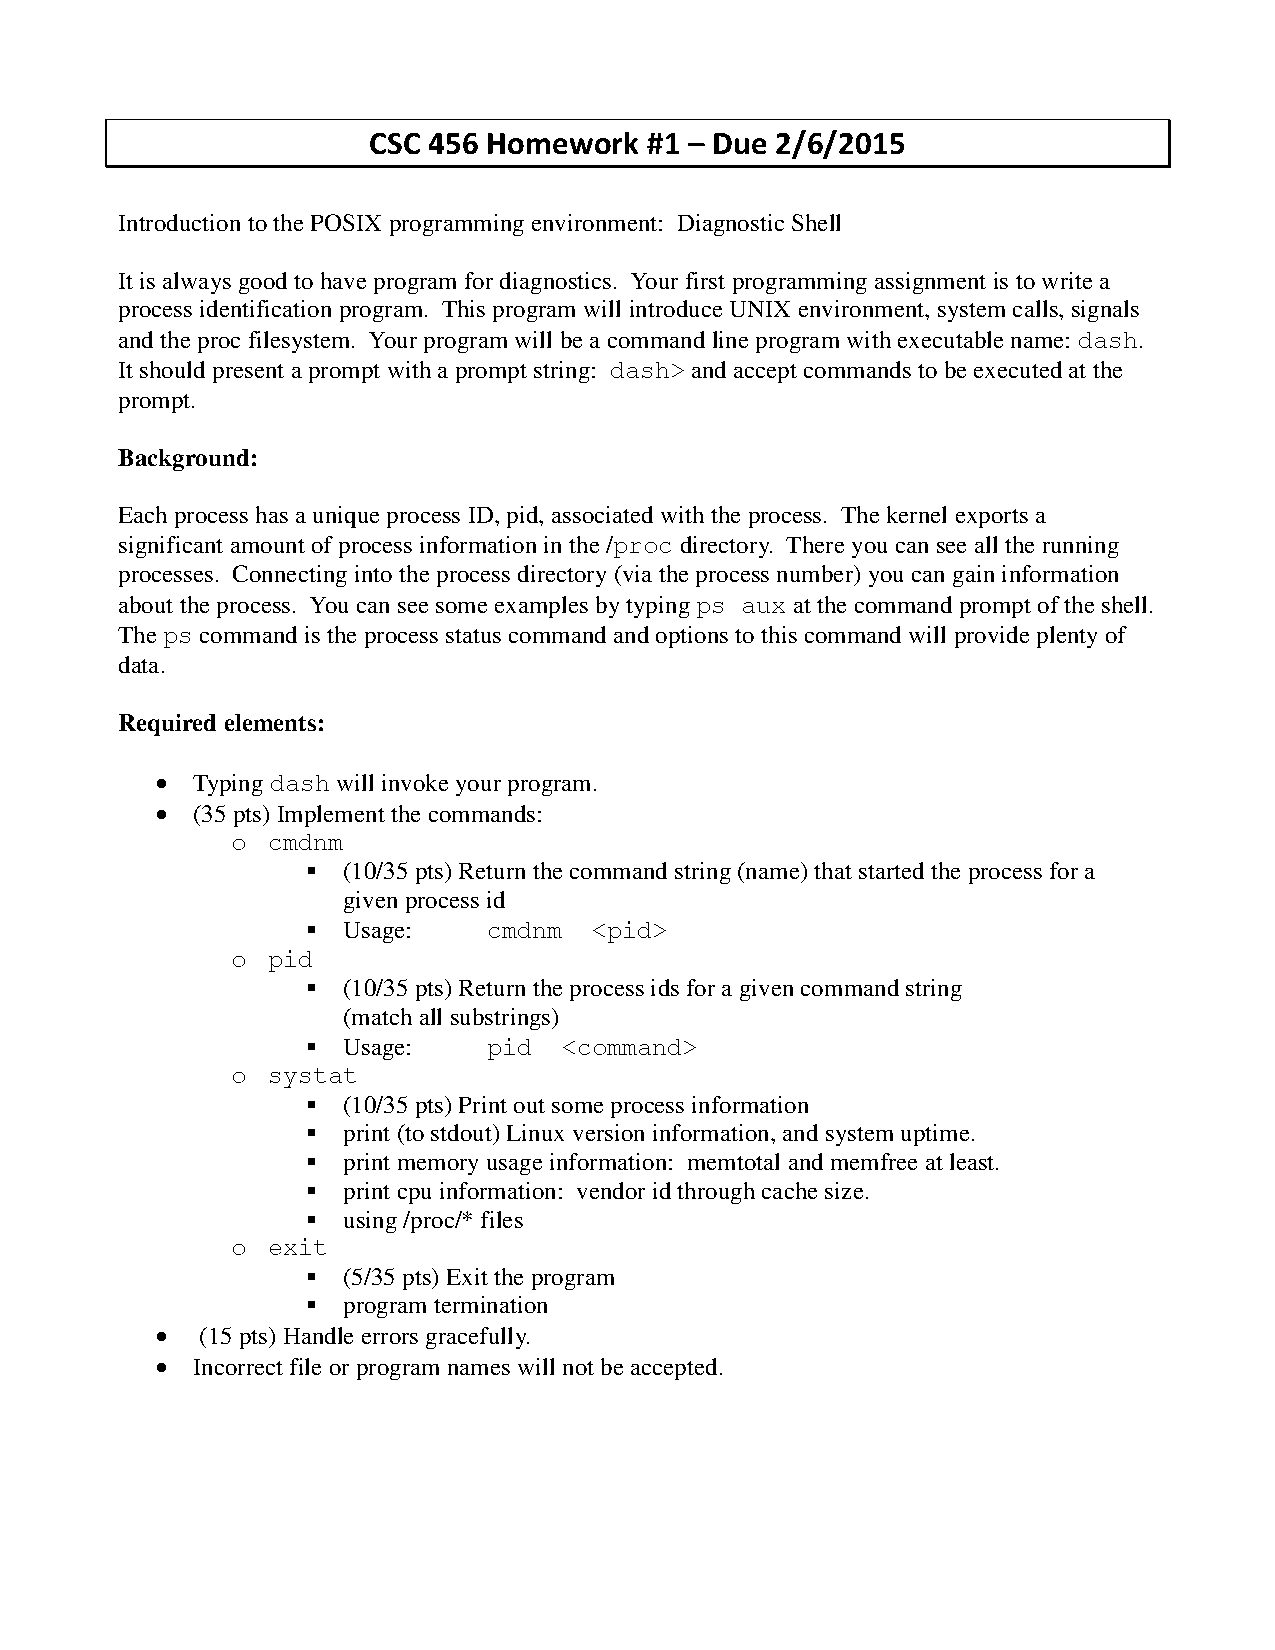
\includepdf[pages={1-4},frame={true}]{csc456_HW1.pdf}


\end{document}